\begin{definition}
    Stan \(j\) jest \textbf{osiągalny} ze stanu \(i\) jeśli istnieje \(n \geq 0\) takie, że
    \(\pars{P^n}_{i, j} > 0\).
\end{definition}

\begin{definition}
    Stany \(i\) oraz \(j\) są \textbf{skomunikowane} jeśli \(i\) jest osiągalne z \(j\) oraz
    \(j\) jest osiągalne z \(i\). Zapisujemy \( i \leftrightarrow j \).
\end{definition}

\begin{definition}
    Łańcuch jest \textbf{nieredukowalny (nieprzywiedlny)} jeśli wszystkie stany są parami skomunikowane.
\end{definition}

\begin{definition}
    Definiujemy \textbf{prawdopodobieństwo pierwszego spotkania w zadanym momencie} \(r_{i, j}^t\) 
    jako 
    \[
        r_{i, j}^t = P(X_t = j \land X_{t-1} \neq j \dots X_{1} \neq j \mid X_0 = i)  
    \]
\end{definition}

\begin{definition}
    Definiujemy \textbf{prawdopodobieństwo pierwszego spotkania} \(r_{i, j}\) 
    jako 
    \[
        r_{i, j} = \sum_{t=1}^{\infty} r_{i,j}^{t}
    \]
\end{definition}

\begin{definition}
    Stan \(i\) jest \textbf{rekurencyjny (powracający)} jeśli \( \sum_{t \geq 1} r_{i, i}^t = 1 \)
    a \textbf{chwilowy} jeśli \( \sum_{t \geq 1} r_{i, i}^t < 1 \). \\
    Mówimy, że łańcuch jest rekurencyjny jeśli każdy jego stan jest rekurencyjny.
\end{definition}
 
 \begin{definition}
    Definiujemy \textbf{oczekiwany czas pierwszego spotkania} \(h_{i, j} = \sum_{t \geq 1} t \cdot r_{i, j}^t\)
 \end{definition}

\begin{definition}
   Rekurencyjny stan \(i\) jest \textbf{pozytywnie rekurencyjny} jeśli \(h_{i, i} < \infty\),
   w przeciwnym wypadku jest \textbf{null rekurencyjny}.
\end{definition}

\begin{definition}
    Stan \(i\) jest \textbf{okresowy} jeśli istnieje \(\Delta \in \natural, \Delta > 1 \) takie, że
        \[
            \forall s : P(X_s = i \mid X_0 = i) \neq 0 \Rightarrow \Delta \mid s  
        \]
        oraz
        \[
            \exists s : P(X_s = i \mid X_0 = i) \neq 0
        \]
    Łańcuch jest okresowy jeśli posiada co najmniej jeden stan okresowy.
    Stan lub łańcuch, które nie są okresowe nazywamy nieokresowymi.
\end{definition}
\begin{figure}[H]
    \centering
    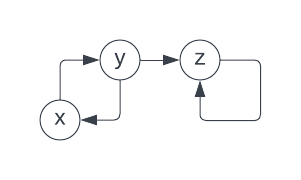
\includegraphics{img/markov-chains/periodic-states-example.png}
    \caption{Przykład okresowości -- stany \( x \) i \( y \) są okresowe, stan \( z \) nie jest}
\end{figure}


\begin{definition}
   Stan jest \textbf{ergodyczny} jeśli jest nieokresowy i pozytywnie rekurencyjny.
   Łańcuch jest ergodyczny jeśli każdy jego stan jest ergodyczny.
\end{definition}

\begin{lemma}
    Relacja skomunikowania jest relacją równoważności.
\end{lemma}
\begin{proof} Rozważamy trzy warunki bycia relacją równoważności
    \begin{enumerate}
        \item \( i \leftrightarrow i \) \\
            Możemy dojść z \( i \) do \( i \) w 0 krokach -- \( \pars{P^0}_{i, j} = 1 \)
        
        \item \( i \leftrightarrow j \implies j \leftrightarrow i \) \\
            Koniunkcja jest przemienna, możemy zatem zamienić kolejność warunków w definicji.
        
        \item \( i \leftrightarrow j \land j \leftrightarrow k \implies i \leftrightarrow k \) \\
            Skoro \( i \leftrightarrow j \) to mamy \( n \) dla którego \(\pars{P^n}_{i, j} > 0\).
            
            Podobnie mamy \( m \) dla którego \( \pars{P^m}_{j, k} > 0 \).
            
            W takim razie \( \pars{P^{n+m}} \geq \pars{P^n}_{i, j} \cdot \pars{P^m}_{j, k} > 0 \)
            zatem \( k \) jest osiągalne z \( i \).
            
            Analogicznie pokazujemy, że \( i \) jest osiągalne z \( k \), czyli stany te są skomunikowane.
            
    \end{enumerate}
\end{proof}

\begin{lemma}
    W skończonym procesie Markowa:
    \begin{enumerate}
        \item istnieje co najmniej jeden stan rekurencyjny
        \item każdy stan rekurencyjny jest pozytywnie rekurencyjny
    \end{enumerate}
    
\end{lemma}
\begin{proof} \( \) \\
    \begin{enumerate}
        \item Załóżmy nie wprost, że wszystkie stany są chwilowe.
        
            Niech \( Y_1, \dots, Y_n \) będą zmiennymi losowymi liczącymi liczbę powrotów do każdego ze stanów.
            
            Zmienne te mają rozkład geometryczny -- jeśli wychodzimy z \(i\)-tego stanu to z prawdopodobieństwem \(p = \sum_{i = 1}^\infty r_{i, i}^t \) wracamy kiedyś do \( i \) (co liczmy jako porażkę) a z prawdopodobieństwem \( 1 - p \) nigdy już nie wracamy do tego stanu (co liczymy jako sukces).
            
            Ponieważ z definicji \( p < 1 \) to \( 1 - p > 0 \)
            zatem
            \[
                \forall_i : \expected{Y_i} \in \real
            \]
            
            Z drugiej jednak strony łańcuch trwa nieskończenie długo, czyli
            \[
                \infty = \expected{\sum_i Y_i} = \sum_i \expected{Y_i}
            \]
            co nam daje sprzeczność.
        
        \item 
        
    \end{enumerate}
\end{proof}

Z lematu tego wysuwamy poniższy wniosek:
\begin{lemma}
    Skończony, nieredukowalny, nieokresowy łańcuch Markowa jest ergodyczny
\end{lemma}

\begin{lemma}
    Jeśli stan \(x\) jest rekurencyjny to
    wszystkie stany w tej samej klasie skomunikowania również są rekurencyjne.
\end{lemma}
\begin{proof}
    Wybierzmy dowolny stan \( y \) w tej samej klasie skomunikowania co \( x \).
    Pokażemy, że jest on rekurencyjny.
    
    Rozważmy zachowanie naszego łańcucha na stanach \( x \) oraz \( y \).
    Możliwe jest kilka zdarzeń:
    \begin{enumerate}
        \item Wychodząc ze stanu \( x \) wracamy do \( x \) zanim napotkamy \( y \) -- z prawdopodobieństwem \( p \)
        
        \item Wychodząc ze stanu \( x \) zanim wrócimy do \( x \) to napotykamy \( y \) \\
            Ponieważ \( x \) jest rekurencyjny to to zdarzenie ma szansę \( 1 - p \)
            
        \item Wychodząc ze stanu \( y \) wracamy do \( y \) zanim napotkamy \( x \) -- z prawdopodobieństwem \( q \)
        \item Wychodząc ze stanu \( y \) napotkamy \( x \) zanim wrócimy do \( y \) -- z prawdopodobieństwem \( r \)
        
        \item Wychodząc ze stanu \( y \) nigdy nie wracamy ani do \( x \) ani do \( y \) -- z prawdopodobieństwem \( s \)
    \end{enumerate}
    Oczywiście \( q + r + s = 1 \) bo zdarzenia te wyczerpują wszystkie możliwe zachowania łańcucha.
    Ponadto ze skomunikowania mamy \( 1 - p > 0, r > 0 \)
    Poniżej przedstawiamy graficzną reprezentację opisanych zdarzeń.
    
    \begin{figure}[H]
        \centering
        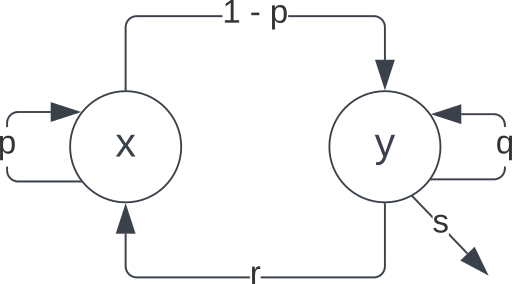
\includegraphics{img/markov-chains/recurrent-communicated-a-priori.png}
        \caption{Ilustracja przejść między możliwymi sytuacjami}
    \end{figure}
    
    Jak się dobrze przyjrzymy to dojdziemy do wniosku, że \( s = 0 \). Dlaczego ?
    Bo inaczej z prawdopodobieństwem co najmniej \( (1-p) \cdot s \) wychodząc z \( x \)
    nigdy już do niego nie wrócimy, co jest sprzeczne z założeniem że jest on rekurencyjny.
    
    W takim razie \(s = 0\), a co za tym idzie \(r = 1 - q\), możemy zatem uprościć nieco nasz rysunek:
    
    \begin{figure}[H]
        \centering
        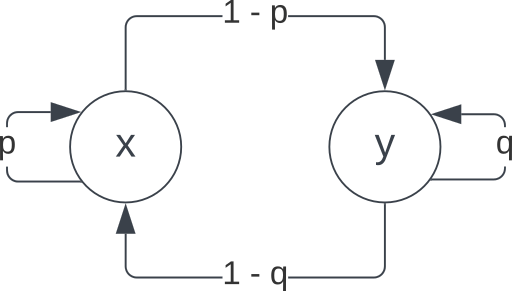
\includegraphics{img/markov-chains/recurrent-communicated-a-posteriori.png}
        \caption{Ilustracja przejść między możliwymi sytuacjami po uproszczeniu}
    \end{figure}
    
    Aby pokazać, że \( y \) jest rekurencyjny pokażemy, że prawdopodobieństwo na to, że wychodząc z \(y \) od pewnego momentu nigdy już nie wrócimy do \( y \) jest zerowe.
    Do \( y \) nigdy nie wracamy, jeśli po skończonej liczbie kroków trafiamy do \( x \) a następnie
    nigdy już nie wracamy do \( y \).
    
    Innymi słowy przechodzimy nieskończenie wiele razy po pętli \( x \rightarrow x \) za każdym razem z prawdopodobieństem \( p \), a szansa na takie zdarzenie wynosi \( \lim_{n \rightarrow \infty} p^n = 0 \)
    
    
    
    

\end{proof}

